\chapter{Gráficos do Experimento 2 da Etapa 1}
As Figuras \ref{fig:graphGC2-01}-\ref{fig:graphGC2-10} apresentam a evolução do VPL da melhor solução, da pior solução e a média da população das dez execuções do Algoritmo Genético Geracional Clássico durante o Experimento 2 da Etapa 1 ($AG^{CC-2}$).

\begin{figure}[H]
\centering
\includegraphics[scale=1]{apxB/aggc/1}
\caption{Evoluçao do VPL para a primeira execução da versão clássica Algoritmo Genético Geracional com o novo operador de recombinação.}
\label{fig:graphGC2-01}
\end{figure}

\begin{figure}[H]
\centering
\includegraphics[scale=1]{apxB/aggc/2}
\caption{Evoluçao do VPL para a primeira execução da versão clássica Algoritmo Genético Geracional com o novo operador de recombinação.}
\label{fig:graphGC2-02}
\end{figure}

\begin{figure}[H]
\centering
\includegraphics[scale=1]{apxB/aggc/3}
\caption{Evoluçao do VPL para a primeira execução da versão clássica Algoritmo Genético Geracional com o novo operador de recombinação.}
\label{fig:graphGC2-03}
\end{figure}

\begin{figure}[H]
\centering
\includegraphics[scale=1]{apxB/aggc/4}
\caption{Evoluçao do VPL para a quarta execução da versão clássica Algoritmo Genético Geracional com o novo operador de recombinação.}
\label{fig:graphGC2-04}
\end{figure}

\begin{figure}[H]
\centering
\includegraphics[scale=1]{apxB/aggc/5}
\caption{Evoluçao do VPL para a quinta execução da versão clássica Algoritmo Genético Geracional com o novo operador de recombinação.}
\label{fig:graphGC2-05}
\end{figure}

\begin{figure}[H]
\centering
\includegraphics[scale=1]{apxB/aggc/6}
\caption{Evoluçao do VPL para a sexta execução da versão clássica Algoritmo Genético Geracional com o novo operador de recombinação.}
\label{fig:graphGC2-06}
\end{figure}

\begin{figure}[H]
\centering
\includegraphics[scale=1]{apxB/aggc/7}
\caption{Evoluçao do VPL para a sétima execução da versão clássica Algoritmo Genético Geracional com o novo operador de recombinação.}
\label{fig:graphGC2-07}
\end{figure}

\begin{figure}[H]
\centering
\includegraphics[scale=1]{apxB/aggc/8}
\caption{Evoluçao do VPL para a Oitava execução da versão clássica Algoritmo Genético Geracional com o novo operador de recombinação.}
\label{fig:graphGC2-08}
\end{figure}

\begin{figure}[H]
\centering
\includegraphics[scale=1]{apxB/aggc/9}
\caption{Evoluçao do VPL para a nona execução da versão clássica Algoritmo Genético Geracional com o novo operador de recombinação.}
\label{fig:graphGC2-09}
\end{figure}

\begin{figure}[H]
\centering
\includegraphics[scale=1]{apxB/aggc/10}
\caption{Evoluçao do VPL para a sécima execução da versão clássica Algoritmo Genético Geracional com o novo operador de recombinação.}
\label{fig:graphGC2-10}
\end{figure}

As Figuras \ref{fig:graphRPC2-01}-\ref{fig:graphRPC2-10} apresentam a evolução do VPL da melhor solução, da pior solução e a média da população das dez execuções do Algoritmo Genético de Regime Permanente Clássico durante o Experimento 2 da Etapa 1 ($AG^{RPC-2}$).

\begin{figure}[H]
\centering
\includegraphics[scale=1]{apxB/agrpc/1}
\caption{Evoluçao do VPL para a primeira execução da versão clássica Algoritmo de Regime Permanente com o novo operador de recombinação.}
\label{fig:graphRPC2-01}
\end{figure}

\begin{figure}[H]
\centering
\includegraphics[scale=1]{apxB/agrpc/2}
\caption{Evoluçao do VPL para a segunda execução da versão clássica Algoritmo de Regime Permanente com o novo operador de recombinação.}
\label{fig:graphRPC2-02}
\end{figure}

\begin{figure}[H]
\centering
\includegraphics[scale=1]{apxB/agrpc/3}
\caption{Evoluçao do VPL para a terceira execução da versão clássica Algoritmo de Regime Permanente com o novo operador de recombinação.}
\label{fig:graphRPC2-03}
\end{figure}

\begin{figure}[H]
\centering
\includegraphics[scale=1]{apxB/agrpc/4}
\caption{Evoluçao do VPL para a quarta execução da versão clássica Algoritmo de Regime Permanente com o novo operador de recombinação.}
\label{fig:graphRPC2-04}
\end{figure}

\begin{figure}[H]
\centering
\includegraphics[scale=1]{apxB/agrpc/5}
\caption{Evoluçao do VPL para a quinta execução da versão clássica Algoritmo de Regime Permanente com o novo operador de recombinação.}
\label{fig:graphRPC2-05}
\end{figure}

\begin{figure}[H]
\centering
\includegraphics[scale=1]{apxB/agrpc/6}
\caption{Evoluçao do VPL para a sexta execução da versão clássica Algoritmo de Regime Permanente com o novo operador de recombinação.}
\label{fig:graphRPC2-06}
\end{figure}

\begin{figure}[H]
\centering
\includegraphics[scale=1]{apxB/agrpc/7}
\caption{Evoluçao do VPL para a sétima execução da versão clássica Algoritmo de Regime Permanente com o novo operador de recombinação.}
\label{fig:graphRPC2-07}
\end{figure}

\begin{figure}[H]
\centering
\includegraphics[scale=1]{apxB/agrpc/8}
\caption{Evoluçao do VPL para a oitava execução da versão clássica Algoritmo de Regime Permanente com o novo operador de recombinação.}
\label{fig:graphRPC2-08}
\end{figure}


\begin{figure}[H]
\centering
\includegraphics[scale=1]{apxB/agrpc/9}
\caption{Evoluçao do VPL para a nona execução da versão clássica Algoritmo de Regime Permanente com o novo operador de recombinação.}
\label{fig:graphRPC2-09}
\end{figure}

\begin{figure}[H]
\centering
\includegraphics[scale=1]{apxB/agrpc/10}
\caption{Evoluçao do VPL para a Décima execução da versão clássica Algoritmo de Regime Permanente com o novo operador de recombinação.}
\label{fig:graphRPC2-10}
\end{figure}